\documentclass[12pt]{article}
\usepackage{graphicx}

\begin{document}
\title{Implementation of Reinforcement Learning Algorithms}
\date{February 11, 2015}
\author{Imanol Arrieta Ibarra}
\maketitle

Because of the nature of the problem, performance can either be optimal or not. Optimal if after H time steps we observe a positive reword; not optimal, otherwise. So, to compute when the algorithm is typically achieving optimal performance we will compute local averages and report only those H's for which at 1000 episodes we achieve optimal performance more than $50\%$ of the time. For local averages I refer to the average over 10 episodes. 

\section{UCRL}
\begin{figure}[h]
\centering
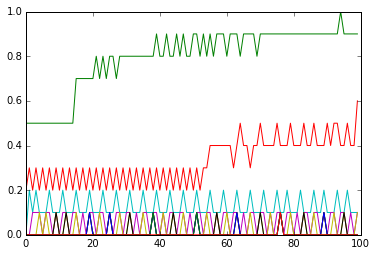
\includegraphics[scale=.4]{Average_Last_Ten.png}
\caption{Average for each ten episodes.}
\label{fig:UCRL}
\end{figure}

As can be seen by figure \ref{fig:UCRL}, only $H=1$(green line) and $H=2$ (red line) achieve typical optimal performance after 1000 episodes. 
\pagebreak
\section{PSRL}
\begin{figure}[h]
\centering
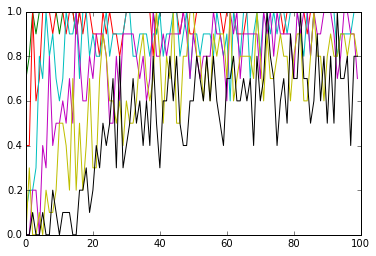
\includegraphics[scale=.4]{Average_Last_Ten_PSRL.png}
\caption{Average for each ten episodes for $H\in\{1,9\}$.}
\label{fig:PSRL}
\end{figure}

\begin{figure}[h]
\centering
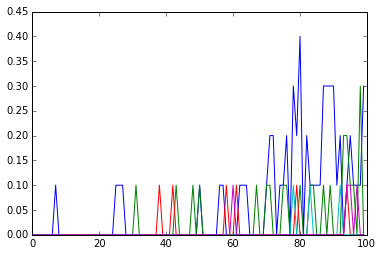
\includegraphics[scale=.4]{Average_Last_Ten_PSRL_rest.png}
\caption{Average for each ten episodes for $H\in\{10,15\}$.}
\label{fig:PSRL_rest}
\end{figure}

Figure \ref{fig:PSRL} shows the local averages for $H\in\{1,9\}$. On the other hand \ref{fig:PSRL_rest} shows the local averages for H greater than $9$. So the maximum H that typically attains optimum is 9. 
\section{Epsilon-PSRL}
\begin{figure}[h]
\centering
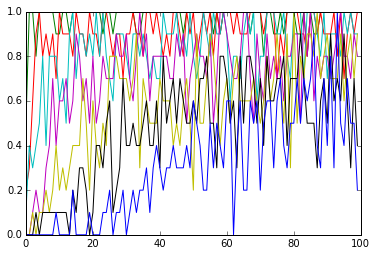
\includegraphics[scale=.4]{Average_Last_Ten_eps.png}
\caption{Average for each ten episodes for $H\in\{1,9\}$.}
\label{fig:eps}
\end{figure}

\begin{figure}[h]
\centering
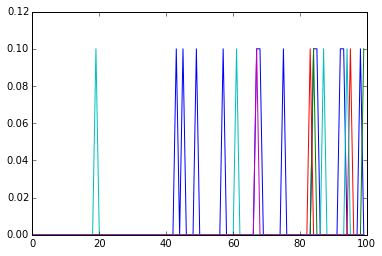
\includegraphics[scale=.4]{Average_Last_Ten_eps_rest.png}
\caption{Average for each ten episodes for $H\in\{10,15\}$.}
\label{fig:eps_rest}
\end{figure}

Figure \ref{fig:eps} shows the local averages for $H\in\{1,11\}$. On the other hand \ref{fig:eps_rest} shows the local averages for H greater than $11$. So the maximum H that typically attains optimum is 11 with the proper epsilon-tuning. 

\end{document}